\section*{LUYỆN TẬP CHUNG 1}

%%==========Bài 1
\begin{bt}
	Với giá trị nào của $x$ thì các căn thức sau xác định
	\begin{multicols}{4}
	\begin{listEX}
	\item $\sqrt{-3x}$.
	\item $\sqrt{2x-4}$.
	\item $\sqrt{7-6x}$.
	\item $\sqrt{-3x+2}$.
	\item $\dfrac{x}{x-2}+\sqrt{x-2}$.
	\item $\dfrac{x}{x+2}+\sqrt{x-2}$.
	\item $\sqrt{\dfrac{1}{3-2x}}$.
	\item $\sqrt{\dfrac{-2}{x+1}}$.
	\item $\sqrt{\dfrac{4x^2}{3x-1}}$.
	\item $\sqrt{\dfrac{2-3x}{4x^2}}$.
	\end{listEX}
	\end{multicols}
	\loigiai{
	\begin{listEX}
	\item $\sqrt{-3x}$ xác định khi $-3x \ge 0$ suy ra $x \le 0$.
	\item $\sqrt{2x-4}$ xác định khi $2x-4 \ge 0$ hay $2x \ge 4$, suy ra $x \ge 2$.
	\item $\sqrt{7-6x}$ xác định khi $7-6x \ge 0$ hay $6x \le 7$, suy ra $x \le \dfrac{7}{6}$.
	\item $\sqrt{-3x+2}$ xác định khi $-3x+2 \ge 0$ hay $3x \le 2$, suy ra $x \le \dfrac{2}{3}$.
	\item $\dfrac{x}{x-2}+\sqrt{x-2}$ xác định khi $\heva{&x-2 \ne 0\\&x-2 \ge 0} $ hay $\heva{&x\ne 2\\&x \ge 2}$, suy ra $ x>2$.
	\item $\dfrac{x}{x+2}+\sqrt{x-2}$ xác định khi $\heva{&x+2 \ne 0\\&x-2 \ge 0} $ hay $\heva{&x\ne -2\\&x \ge 2}$, suy ra $x \ge 2$.
	\item $\sqrt{\dfrac{1}{3-2x}}$ xác định khi 
	$\dfrac{1}{3-2x} \ge 0$ hay $3-2x>0$, suy ra $x < \dfrac{3}{2}$.
	\item $\sqrt{\dfrac{-2}{x+1}}$ xác định khi 
	$\dfrac{-2}{x+1} \ge 0$ hay $x+1<0$, suy ra $x <-1$.
	\item $\sqrt{\dfrac{4x^2}{3x-1}}$ xác định khi 
	$\dfrac{4x^2}{3x-1} \ge 0$ hay $\hoac{&\heva{&x^2\ge 0\\&3x-1>0}\\&\heva{&x^2= 0\\&3x-1\ne 0}}$, suy ra $\hoac{&\heva{&\forall x \in \mathbb{R} \\&x>\dfrac{1}{3}}\\&\heva{&x=0\\&x \ne \dfrac{1}{3}}}$
	 $\Rightarrow \hoac{&x>\dfrac{1}{3}\\&x=0.}$
	\item $\sqrt{\dfrac{2-3x}{4x^2}}$ xác định khi 
	$\dfrac{2-3x}{4x^2}\ge 0$ hay $\heva{&x \ne 0\\&2-3x \ge 0}$, suy ra $\heva{&x \ne 0\\&x \le \dfrac{2}{3}.}$
	\end{listEX}
	}
\end{bt}

%%==========Bài 2
\begin{bt}
	Có bao nhiêu giá trị nguyên của $x$ để biểu thức $M=\sqrt{x+4}+\sqrt{2-x}$ có nghĩa?
	\loigiai{
	$M$ có nghĩa khi $\heva{&x+4 \ge 0\\&2-x \ge 0} \Rightarrow \heva{&x \ge -4\\&x \le 2.}$\\
	Vì $x \in \mathbb{Z}$ nên $x \in \{-4;-3;-2;-1;0;1;2\}$.\\
	Vậy có $7$ giá trị nguyên của $x$ để biểu thức $M$ có nghĩa.
	}
\end{bt}

%%==========Bài 3
\begin{bt}%[9D1Y9]
	Tính 
	\begin{listEX}[2]
	\item $\sqrt[3]{162}\cdot\sqrt[3]{ - 2}\cdot\sqrt[3]{\dfrac{2}{3}}$;
	\item $\sqrt[3]{2}:\sqrt[3]{16} - \sqrt[3]{22\dfrac{1}{2}}:\sqrt[3]{53\dfrac{1}{3}}$.
	\end{listEX}
	\loigiai
	{
	\begin{listEX}[2]
	\item $-6$;
	\item $-\dfrac{1}{4}$.
	\end{listEX}
	}
\end{bt}

%%==========Bài 4
\begin{bt}%[9D1Y9]
	Tính 
	\begin{listEX}[2]
	\item $\left(\sqrt[3]{3} + \sqrt[3]{2}\right)^3$;
	\item $\left(\sqrt[3]{5} - \sqrt[3]{3}\right)\left(\sqrt[3]{25} + \sqrt[3]{15} + \sqrt[3]{9}\right)$.
	\end{listEX}
	\loigiai
	{
	\begin{listEX}[2]
	\item $5 + 3\sqrt[3]{18} + 3\sqrt[3]{12}$; 
	\item $2.$
	\end{listEX}
	}
\end{bt}

%%==========Bài 5
\begin{bt}%[9D1B9]
	Rút gọn biểu thức 
	\begin{listEX}[2]
	\item $\sqrt[3]{3}\cdot(5\sqrt[3]{18} - 3\sqrt[3]{144}) + \sqrt[3]{5}\cdot\sqrt[3]{50}$;
	\item $(12\sqrt[3]{2} + \sqrt[3]{16} - 2\sqrt[3]{2})\left(5\sqrt[3]{4} - 3\sqrt[3]{\dfrac{1}{2}}\right)$.
	\end{listEX}
	\loigiai
	{
	\begin{listEX}[2]
	\item $2\sqrt[3]{2}$;
	\item $84.$
	\end{listEX}
	}
\end{bt}

%%==========Bài 6
\begin{bt}
	Không dùng MTCT, tính giá trị của biểu thức
	$$A=\sqrt{(1-\sqrt{3})^2}-\sqrt{3}.$$
	\loigiai{
	Ta có $A=\left|1-\sqrt{3}\right|-\sqrt{3}=\left(\sqrt{3}-1\right)-\sqrt{3}=-1. \leftarrow$ Hằng đẳng thức $\sqrt{A^2}=\left|A\right|$.
	}
\end{bt}
%%==========Bài 7
\begin{bt}%[9D1K9]
	Tính $M=\sqrt[3]{5\sqrt{2} + 7} - \sqrt[3]{5\sqrt{2} - 7}$.
	\loigiai
	{
	\allowdisplaybreaks 
	\begin{eqnarray*}
	&&M^3=(5\sqrt{2} + 7) - (5\sqrt{2} - 7) - 3\sqrt[3](5\sqrt{2} + 7)(5\sqrt{2} - 7) \cdot M\\
	&\Leftrightarrow& M^3=14 - 3 M\\
	&\Leftrightarrow& M^3 + 3 M - 14=0\\
	&\Leftrightarrow& \left( M - 2\right)\left( M^2 + 2M + 7\right)=0\\
	&\Leftrightarrow& M - 2=0~\left(\text{vì } M^2 + 2 M + 7=( M + 1)^2 + 6>0\right)\\
	&\Leftrightarrow& M=2.
	\end{eqnarray*}
	}
\end{bt}

%%==========Bài 8
\begin{bt}
	Thực hiện các phép tính:
	\begin{listEX}[4]
	\item $\sqrt{27\cdot 75}$;
	\item $\sqrt{200\cdot 18}$;
	\item $\sqrt{160\cdot 12{,}1}$;
	\item $\sqrt{3{,}6\cdot 25{,}6}$.
	\end{listEX}
	\loigiai{
	\begin{listEX}
	\item $\sqrt{27\cdot 75}=\sqrt{9\cdot 9\cdot 25}=\sqrt{9}\cdot \sqrt{9}\cdot \sqrt{25}=3\cdot 3\cdot 5=45$.
	\item $\sqrt{200\cdot 18}=\sqrt{100\cdot 4\cdot 9}=\sqrt{100}\cdot \sqrt{4}\cdot \sqrt{9}=10\cdot 2\cdot 3=60$.
	\item $\sqrt{160\cdot 12{,}1}=\sqrt{16\cdot 100\cdot 1{,}21}=\sqrt{16}\cdot \sqrt{100}\cdot \sqrt{1{,}21}=4\cdot 10\cdot 1{,}1=44$.
	\item $\sqrt{3{,}6\cdot 25{,}6}=\sqrt{0{,}36\cdot 100\cdot 2{,}56}=\sqrt{0{,}36}\cdot \sqrt{100}\cdot \sqrt{2{,}56}=0{,}6\cdot 10\cdot 1{,}6=9{,}6$.
	\end{listEX} 
	}
\end{bt}

%%==========Bài 9
\begin{bt}
	Thực hiện các phép tính:
	\begin{listEX}[4]
	\item $\sqrt{45}\cdot \sqrt{180}$;
	\item $\sqrt{7}\cdot \sqrt{105}$;
	\item $\sqrt{250}\cdot \sqrt{0,9}$;
	\item $\sqrt{8}\cdot \sqrt{162}$.
	\end{listEX}
	\loigiai{
	\begin{listEX}
	\item $\sqrt{45}\cdot \sqrt{180}=\sqrt{45\cdot 180}=\sqrt{8100}=90$.
	\item $\sqrt{7}\cdot \sqrt{175}=\sqrt{7\cdot 175}=\sqrt{1225}=35$.
	\item $\sqrt{250}\cdot \sqrt{0,9}=\sqrt{250\cdot 0{,}9}=\sqrt{225}=15$.
	\item $\sqrt{8}\cdot \sqrt{162}=\sqrt{8\cdot 162}=\sqrt{1296}=36$.
	\end{listEX}
	}
\end{bt}

%%==========Bài 10
\begin{bt}
	Thực hiện các phép tính:
	\begin{listEX}[2]
	\item $ A=\sqrt{\dfrac{49}{81}} $;
	\item $ B=\dfrac{\sqrt{3+\sqrt{5}}}{\sqrt{2}} .$
	\end{listEX}
	\loigiai{\begin{listEX}
	\item Ta có $A=\sqrt{\dfrac{49}{81}}=\dfrac{\sqrt{49}}{\sqrt{81}}=\dfrac{7}{9}.$
	\item Ta có $B=\sqrt{\dfrac{3+\sqrt{5}}{2}}=\sqrt{\dfrac{6+2\sqrt{5}}{4}}=\dfrac{\sqrt{5+2\sqrt{5}+1}}{\sqrt{4}}=\dfrac{\sqrt{\left(\sqrt{5}+1\right)^2}}{2}=\dfrac{\sqrt{5}+1}{2}.$
	\end{listEX}}
\end{bt}

%%==========Bài 11
\begin{bt}
	Rút gọn các biểu thức sau
	\begin{listEX}[2]
	\item $\sqrt{13+4\sqrt{3}}+2\sqrt{7-4\sqrt{3}}$.
	\item $ (\sqrt{10}-\sqrt{2})\cdot\sqrt{3+\sqrt{5}}. $
	\end{listEX}	
	\loigiai{
	\begin{listEX}
	\item $\sqrt{13+4\sqrt{3}}+2\sqrt{7-4\sqrt{3}}=\sqrt{(1+2\sqrt{3})^2}+2\sqrt{(2-\sqrt{3})^2} = 1+2\sqrt{3} +2(2-\sqrt{3})=5$.
	\item $ (\sqrt{10}-\sqrt{2})\cdot\sqrt{3+\sqrt{5}} = (\sqrt{5}-1)\cdot\sqrt{6+2\sqrt{5}}=(\sqrt{5}-1)\cdot\sqrt{(\sqrt{5}+1)^2} = (\sqrt{5}-1)(\sqrt{5}+1)=4 $.
	\end{listEX}
	}
\end{bt}

%%==========Bài 12
\begin{bt}
	Thực hiện các phép tính:
	\begin{listEX}[3]
	\item $ A=\sqrt{98}\colon\sqrt{2} $;
	\item $ B=\left(\sqrt{48}-\sqrt{27}+\sqrt{3}\right)\colon \sqrt{3} $;
	\item $ C=\left(5\sqrt{3}+3\sqrt{5}\right)\colon\sqrt{15}. $
	\end{listEX}
	\loigiai{
	\begin{listEX}
	\item Ta có $ A=\sqrt{98}\colon\sqrt{2}=\sqrt{98\colon 2}=\sqrt{49}=7. $
	\item Ta có $ B=\left(\sqrt{48}-\sqrt{27}+\sqrt{3}\right)\colon \sqrt{3}=\sqrt{48:3}-\sqrt{27:3}+\sqrt{3:3}=\sqrt{16}-\sqrt{9}+1=2. $
	\item $C=\left(5\sqrt{3}+3\sqrt{5}\right)\colon\sqrt{15}=\left(5\sqrt{3}+3\sqrt{5}\right):\left( \sqrt{5}\cdot\sqrt{3}\right) =\dfrac{5\sqrt{3}}{\sqrt{5}\cdot\sqrt{3}}+\dfrac{3\sqrt{5}}{\sqrt{5}\cdot\sqrt{3}}=\sqrt{5}+\sqrt{3}. $
	\end{listEX}
	}
\end{bt}

%%==========Bài 13
\begin{bt}
	Tính
	\begin{listEX}[2]
	\item $\left(2+\sqrt{5}\right)\left(2-\sqrt{5}\right)$;
	\item $\left(\sqrt{5}+\sqrt{2}\right)\left(\sqrt{5}-\sqrt{2}\right)$.
	\end{listEX}
	\loigiai{
	Sử dụng hằng đẳng thức của hiệu hai bình phương, ta có
	\begin{listEX}
	\item $\left(2+\sqrt{5}\right)\left(2-\sqrt{5}\right)=2^2-\left(\sqrt{5}\right)^2=4-5=-1$.
	\item $\left(\sqrt{5}+\sqrt{2}\right)\left(\sqrt{5}-\sqrt{2}\right)=\left(\sqrt{5}\right)^2-\left(\sqrt{2}\right)^2=5-2=3$.
	\end{listEX}
	}
\end{bt}

%%==========Bài 14
\begin{bt}
	Rút gọn các biểu thức sau
	\begin{listEX}[2]
	\item $\sqrt{\left(\sqrt{3}-\sqrt{2}\right)^2}+\sqrt{\left(1-\sqrt{2}\right)^2}$;
	\item $\sqrt{\left(\sqrt{7}-3\right)^2}+\sqrt{\left(\sqrt{7}+3\right)^2}$.
	\end{listEX}
	\loigiai{
	\begin{listEX}
	\item $\sqrt{\left(\sqrt{3}-\sqrt{2}\right)^2}+\sqrt{\left(1-\sqrt{2}\right)^2}=\left|\sqrt{3}-\sqrt{2}\right|+\left|1-\sqrt{2}\right|=\sqrt{3}-\sqrt{2}+\sqrt{2}-1=\sqrt{3}-1$;
	\item $\sqrt{\left(\sqrt{7}-3\right)^2}+\sqrt{\left(\sqrt{7}+3\right)^2}=\left|\sqrt{7}-3\right|+\left|\sqrt{7}+3\right|=3-\sqrt{7}+\sqrt{7}+3=6$.
	\end{listEX}
	}
\end{bt}

%%==========Bài 15
\begin{bt}
	Thực hiện phép tính
	\begin{listEX}[2]
	\item $\sqrt{3}\left(\sqrt{192}-\sqrt{75}\right)$;
	\item $\dfrac{-3\sqrt{18}+5\sqrt{50}-\sqrt{128}}{7\sqrt{2}}$.
	\end{listEX}
	\loigiai{
	\begin{listEX}
	\item $\sqrt{3}\left(\sqrt{192}-\sqrt{75}\right)=\sqrt{3}\left(\sqrt{3\cdot 64}-\sqrt{3\cdot 25}\right)=\sqrt{3}\left(8\sqrt{3}-5\sqrt{3}\right)=\sqrt{3}\cdot 3 \sqrt{3} =3\cdot 3=9$.
	\item $\begin{aligned}[t]
	\dfrac{-3\sqrt{18}+5\sqrt{50}-\sqrt{128}}{7\sqrt{2}}&=\dfrac{-3\sqrt{2\cdot 9}+5\sqrt{2\cdot 25}-\sqrt{2\cdot 64}}{7\sqrt{2}}=\dfrac{-9\sqrt{2}+25\sqrt{2}-8\sqrt{2}}{7\sqrt{2}}\\&=\dfrac{8\sqrt{2}}{7\sqrt{2}}=\dfrac{8}{7}.
	\end{aligned}$
	\end{listEX}
	}
\end{bt}

%%==========Bài 16
\begin{bt}
	Chứng minh rằng
	\begin{listEX}[2]
	\item $\left(1-\sqrt{2}\right)^2=3-2\sqrt{2}$;
	\item $\left(\sqrt{3}+\sqrt{2}\right)^2=5+2\sqrt{6}$.
	\end{listEX}
	\loigiai{
	\begin{listEX}
	\item $\left(1-\sqrt{2}\right)^2=1^2-2\cdot 1 \cdot \sqrt{2} +\left(\sqrt{2}\right)^2=3-2\sqrt{2} \Rightarrow$ (đpcm).
	\item $\left(\sqrt{3}+\sqrt{2}\right)^2=\left(\sqrt{3}\right)^2+2\cdot \sqrt{3}\cdot \sqrt{2}+\left(\sqrt{2}\right)^2=3+2\sqrt{6}+2=5+2\sqrt{6}\Rightarrow$ (đpcm).
	\end{listEX}
	}
\end{bt}

%%==========Bài 17
\begin{bt}
	Tính
	\begin{listEX}[2]
	\item $\sqrt{10{,}6^2-5{,}6^2}$;
	\item $\sqrt{29+12\sqrt{5}}+\sqrt{29-12\sqrt{5}}$;
	\item $\dfrac{\sqrt{10}+\sqrt{26}}{2\sqrt{5}+\sqrt{52}}$;
	\item $\left(1+\sqrt{2}-\sqrt{3}\right)\left(1-\sqrt{2}+\sqrt{3}\right)$;
	\item $\left(\sqrt{5+\sqrt{21}}+\sqrt{5-\sqrt{21}}\right)^2$;
	\item $\dfrac{3\sqrt{2}-\sqrt{3}-\sqrt{6}+\sqrt{16}}{\sqrt{2}-\sqrt{3}+\sqrt{4}}$.
	\end{listEX}
	\loigiai{	
	\begin{listEX}
	\item $\sqrt{5{,}3^2-2{,}8^2}=\sqrt{8{,}1\cdot 2{,}5}=\sqrt{81\cdot 100\cdot 0{,}25}=9\cdot 10\cdot 0{,}5=45$.
	\item $\begin{aligned}[t]
	\sqrt{29+12\sqrt{5}}+\sqrt{29-12\sqrt{5}} &= \sqrt{\left(3+2\sqrt{5}\right)^2}+\sqrt{\left(3-2\sqrt{5}\right)^2}\\
	&= \left(3+2\sqrt{5}\right)+\left(2\sqrt{5}-3\right)=4\sqrt{5}.
	\end{aligned}$
	\item $\dfrac{\sqrt{10}+\sqrt{26}}{2\sqrt{5}+\sqrt{52}}=\dfrac{\sqrt{2}\cdot \left(\sqrt{5}+\sqrt{13}\right)}{2\cdot \left(\sqrt{5}+\sqrt{13}\right)}=\dfrac{\sqrt{2}}{2}$.
	\item $\left(1+\sqrt{2}-\sqrt{3}\right)\left(1-\sqrt{2}+\sqrt{3}\right)=1-\left(\sqrt{2}-\sqrt{3}\right)^2=1-\left(5-2\sqrt{6}\right)=2\sqrt{6}-4$.
	\item $\begin{aligned}[t]
	\left(\sqrt{5+\sqrt{21}}+\sqrt{5-\sqrt{21}}\right)^2 &= 5+\sqrt{21}+2\cdot \sqrt{5+\sqrt{21}}\cdot \sqrt{5-\sqrt{21}}+5-\sqrt{21}\\
	&= 10+2\sqrt{\left(5+\sqrt{21}\right)\left(5-\sqrt{21}\right)}\\
	&= 10+2\sqrt{4}=14.
	\end{aligned}$
	\item $\begin{aligned}[t]
	\dfrac{3\sqrt{2}-\sqrt{3}-\sqrt{6}+\sqrt{16}}{\sqrt{2}-\sqrt{3}+\sqrt{4}} &=\dfrac{\sqrt{4}-\sqrt{6}+\sqrt{8}+\sqrt{2}-\sqrt{3}+\sqrt{4}}{\sqrt{2}-\sqrt{3}+\sqrt{4}}\\
	&=\dfrac{\sqrt{2}\left(\sqrt{2}-\sqrt{3}+\sqrt{4}\right)+\sqrt{2}-\sqrt{3}+\sqrt{4}}{\sqrt{2}-\sqrt{3}+\sqrt{4}}\\
	&=\sqrt{2}+1.
	\end{aligned}$
	\end{listEX}
	}
\end{bt}

%%==========Bài 18
\begin{bt}
	Rút gọn các biểu thức sau:
	\begin{listEX}[2]
	\item $\sqrt{x^4-4x^2+4}-x^2$.
	\item $\dfrac{\sqrt{x^4-2x^2+1}}{x+1}$, với $x>1$.
	\item $\dfrac{\sqrt{4x^{2}+4x+1}}{4x^{2}-1}$ với $x>-\dfrac{1}{2}$.
	\item $ 9+x+\sqrt{4-4x+x^{2}}$ với $x<2$.
	\end{listEX}
	\loigiai{
	\begin{listEX}
	\item $\sqrt{x^4+4x^2+4}-x^2=\sqrt{\left(x^2+2\right)^2}-x^2 =x^2+2-x^2=2$, ($x^2+2>0$).
	\item $\dfrac{\sqrt{x^4-2x^2+1}}{x+1}=\dfrac{\sqrt{\left(x^2-1\right)^2}}{x+1}$, ($x^2-1>0$)
	\\ $=\dfrac{x^2-1}{x+1}=\dfrac{(x-1)(x+1)}{x+1}=x-1$.
	\item $A=\dfrac{\sqrt{4x^{2}+4x+1}}{4x^{2}-1}$
	$=\dfrac{\sqrt{(2x+1)^2}}{(2x+1)(2x-1)}$
	$=\dfrac{|2x+1|}{(2x+1)(2x-1)}$.\\
	Do $x>-\dfrac{1}{2}$ nên $2x+1>0$. 
	\\Suy ra $A=\dfrac{2x+1}{(2x+1)(2x-1)}=\dfrac{1}{2x-1}$.
	\item $B=9+x+\sqrt{4-4x+x^{2}}=9+x+\sqrt{(2-x)^2}=9+x+|2-x|$.\\
	Do $x<2$ nên $2-x>0$.\\
	Suy ra $B=9+x+2-x=11$.
	\end{listEX} 
	}
\end{bt}

%%==========Bài 19
\begin{bt}
	Rút gọn các biểu thức sau
	\begin{listEX}[2]
	\item $\sqrt[3]{(-x-1)^{3}}$;
	\item $\sqrt[3]{8 x^{3}-12 x^{2}+6 x-1}$.
	\end{listEX}
	\loigiai{
	\begin{listEX}
	\item $\sqrt[3]{(-x-1)^{3}}=-x-1$.
	\item $\sqrt[3]{8 x^{3}-12 x^{2}+6 x-1}=\sqrt[3]{(2x-1)^3}=2x-1$.
	\end{listEX}
	}
\end{bt}

%%==========Bài 20
\begin{bt}
	Tìm $x$ biết:
	\begin{listEX}[2]
	\item $\sqrt{x^2}=1$.
	\item $\sqrt{4x^2-4x+1}=3$.
	\item	$\sqrt{x^2-4x+4}=3$.
	\item $\sqrt{x^2+2x+1}+\sqrt{x^2+4x+4}=3x$.
	\end{listEX}
	\loigiai{
	\begin{listEX}
	\item $\sqrt{x^2}=1 \Rightarrow |x|=1 \Rightarrow x= \pm 1$.
	\item $\sqrt{4x^2-4x+1}=3 \Rightarrow \sqrt{(2x-1)^2}=3\Rightarrow |2x-1|=3 \Rightarrow \hoac{&x=2\\&x=-1.}$
	\item $\sqrt{x^2-4x+4}=3
	\Rightarrow \sqrt{(x-2)^2}=3
	\Rightarrow \left|x-2 \right|=3
	\Rightarrow \hoac{&x=5\\&x=-1.} $
	\item $\sqrt{x^2+2x+1}+\sqrt{x^2+4x+4}=3x$ 
	$\Rightarrow \sqrt{(x+1)^2}+\sqrt{x+2)^2}=3x
	\Rightarrow |x+1|+|x+2|=3x.$\hfill (1)\\
	Vì $|x+1|+|x+2|\ge 0$ nên $x\ge 0$
	$\Rightarrow x+1>0$ và $x+2>0$.\\ Do đó
	$$(1)\Rightarrow x+1+x+2=3x\Rightarrow x=3\,\,\text{(thỏa mãn)}.$$
	Vậy nghiệm của phương trình là $x=3$.
	\end{listEX} 
	}
\end{bt}
%%==========Bài 21
\begin{bt}%[9D1K9]
	Tìm $x$ biết 
	\begin{listEX}[2]
	\item $2\sqrt[3]{27x} + \dfrac{1}{7}\sqrt[3]{ - 343x} + \sqrt[3]{ - 729x}=2$;
	\item $\sqrt[3]{x^3 - 9x^2}=x - 3$.
	\end{listEX}
	\loigiai
	{
	\begin{listEX}[2]
	\item $-\dfrac{1}{8}$;
	\item $1$.
	\end{listEX}
	}
\end{bt}

%%==========Bài 22
\begin{bt}
	Rút gọn các biểu thức
	\begin{listEX}
	\item $A=\sqrt{(a-1)^2(2a+1)^2}$ với $a>1$;
	\item $B=\sqrt{(b-1)(b+7)+16}$ với $b<-3$;
	\item $C=\sqrt{c^2+10c+25}-\sqrt{c^2-10c+5}$ với $-5\le c\le 5$;
	\item $D=\dfrac{1-d}{\sqrt{d^2-2d+1}}+\dfrac{\sqrt{d^2-4d+4}}{d-2}$ với $d>2$.
	\end{listEX}
	\loigiai{
	\begin{listEX}
	\item $A=\sqrt{(a-1)^2}\cdot \sqrt{(2a+1)^2}=(a-1)(2a+1)$.
	\item $B=\sqrt{b^2+6b+9}=\sqrt{(b+3)^2}=-(b+3)$.
	\item $C=\sqrt{(c+5)^2}-\sqrt{(c-5)^2}=(c+5)-(5-c)=2c$.
	\item $D=\dfrac{1-d}{\sqrt{(d-1)^2}}+\dfrac{\sqrt{(d-2)^2}}{d-2}=\dfrac{1-d}{d-1}+\dfrac{d-2}{d-2}=(-1)+1=0$.
	\end{listEX}
	}
\end{bt}

%%==========Bài 23
\begin{bt}
	Rút gọn các biểu thức sau:
	\begin{listEX}[2]
	\item $ \sqrt{\dfrac{(x-1)^2}{16}} $ với $ x \ge 1 $;
	\item $ \sqrt{\dfrac{x^4}{(a-1)^2}} $ với $ a < 1 $.
	\end{listEX}
	\loigiai{
	\begin{listEX}
	\item Vì $ (x-1)^2 \ge 0 $ và $ 16 > 0 $ nên ta có $$ \sqrt{\dfrac{(x-1)^2}{16}} = \dfrac{\sqrt{(x-1)^2}}{\sqrt{16}} = \dfrac{|x-1|}{4} \overset{\text{ vì }x\ge 1}{=} \dfrac{x-1}{4}. $$ 
	\item Vì $ x^4 \ge 0 $ và $ (a-1)^2 > 0 $ nên ta có
	\[ \sqrt{\dfrac{x^4}{(a-1)^2}} = \dfrac{\sqrt{x^4}}{\sqrt{(a-1)^2}} = \dfrac{x^2}{|a-1|} \overset{\text{vì }a < 1}{=} \dfrac{x^2}{1-a}. \]
	\end{listEX}
	}
\end{bt}

%%==========Bài 24
\begin{bt}
	Rút gọn các biểu thức sau:
	\begin{listEX}[2]
	\item $ \dfrac{\sqrt{27(x-5)^2}}{\sqrt{3}} $ với $ x\ge5 $;
	\item $ \dfrac{\sqrt{(x-4)^4}}{\sqrt{9(x-4)^2}} $ với $ x < 4 $.
	\end{listEX}
	\loigiai{
	\begin{listEX}
	\item Với $ x \ge 5 $ ta có
	\[ \dfrac{\sqrt{27(x-5)^2}}{\sqrt{3}} = \sqrt{\dfrac{27(x-5)^2}{3}} = \sqrt{9(x-5)^2} = \sqrt{9}\cdot\sqrt{(x-5)^2} = 3\cdot|x-5| \overset{\text{ vì } x\ge5}{=} 3(x-5). \]
	\item Với $ x < 4 $ ta có
	\[ \dfrac{\sqrt{(x-4)^4}}{\sqrt{9(x-4)^2}} = \sqrt{\dfrac{(x-4)^4}{9(x-4)^2}} = \sqrt{\dfrac{(x-4)^2}{9}} = \dfrac{\sqrt{(x-4)^2}}{\sqrt{9}} = \dfrac{|x-4|}{3} \overset{\text{ vì } x < 4}{=} \dfrac{4-x}{3}. \]
	\end{listEX}	
	}
\end{bt}

%%==========Bài 25
\begin{bt}
	Rút gọn các biểu thức:
	\begin{multicols}{2}
	\begin{listEX}
	\item $ A=\sqrt{\dfrac{a^2}{b}}\cdot \sqrt{\dfrac{a^6}{b^3}} $, với $ b>0 $;
	\item $ B=b^5\sqrt{\dfrac{a^2+6a+9}{b^8}}. $
	\end{listEX}
	\end{multicols}
	\loigiai{
	\begin{listEX}
	\item Ta sử dụng quy tắc nhân hai căn bậc hai rồi biến đổi tiếp \[A=\sqrt{\dfrac{a^2}{b}}\cdot \sqrt{\dfrac{a^6}{b^3}}=\sqrt{\dfrac{a^2}{b}\cdot\dfrac{a^6}{b^3}}=\sqrt{\dfrac{a^8}{b^4}}=\dfrac{\sqrt{a^8}}{\sqrt{b^4}}=\dfrac{a^4}{b^2}.\]
	\item Ta biến đổi
	\begin{align*}
	B&=b^5\cdot\sqrt{\dfrac{\left(a+3\right)^2}{b^8}}=b^5\cdot\dfrac{\sqrt{\left(a+3\right)^2}}{\sqrt{b^8}}=b^5\cdot\dfrac{|a+3|}{b^4}=b\cdot|a+3|\\
	&=\heva{&b\cdot(a+3)&&\text{nếu } a\ge -3\\&-b\cdot(a+3)&&\text{nếu } a<-3.}
	\end{align*}
	\end{listEX}
	}
\end{bt}

%%==========Bài 26
\begin{bt}
	Rút gọn biểu thức với điều kiện đã cho và tính giá trị của nó:
	\begin{listEX}
	\item $ \sqrt{\dfrac{x-2\sqrt{x}+1}{x+2\sqrt{x}+1}} $ với $ x\ge0 $; tính giá trị tại $ x = 4 $.
	\item $ \sqrt{\dfrac{(x-2)^4}{(3-x)^2}} + \dfrac{x^2-1}{x-3} $ với $ x<3 $; tính giá trị tại $ x = 0{,}5 $.
	\end{listEX}
	\loigiai{
	\begin{listEX}
	\item Với $ x \ge 0 $ ta có
	\[ \sqrt{\dfrac{x-2\sqrt{x}+1}{x+2\sqrt{x}+1}} = \sqrt{\dfrac{(\sqrt{x}-1)^2}{(\sqrt{x}+1)^2}} = \dfrac{\sqrt{(\sqrt{x}-1)^2}}{\sqrt{(\sqrt{x}+1)^2}} = \dfrac{|\sqrt{x}-1|}{|\sqrt{x}+1|} = \dfrac{|\sqrt{x}-1|}{\sqrt{x}+1}. \]
	Thay $ x = 4 $ vào ta có
	\[ \dfrac{|\sqrt{4}-1|}{\sqrt{4}+1} = \dfrac{1}{3}. \]
	\item Với $ x < 3 $ ta có
	\begin{align*}
	\sqrt{\dfrac{(x-2)^4}{(3-x)^2}} + \dfrac{x^2-1}{x-3} = \dfrac{\sqrt{(x-2)^4}}{\sqrt{(3-x)^2}} + \dfrac{x^2-1}{x-3}& = \dfrac{(x-2)^2}{|3-x|} + \dfrac{x^2-1}{x-3}\\ &= \dfrac{x^2-4x+4}{3-x} - \dfrac{x^2-1}{3-x}\\ & = \dfrac{-4x+5}{3-x}.
	\end{align*}
	Thay $ x = 0{,}5 $ vào ta có
	\[ \dfrac{-4\cdot0{,}5+5}{3-0{,}5} = \dfrac{6}{5}. \]
	\end{listEX}	
	}
\end{bt}

%%==========Bài 27
\begin{bt}
	Phân tích các biểu thức sau thành nhân tử
	\begin{listEX}
	\item $A=\sqrt{x^2-16}+\sqrt{x^2-4x}$ với $x>4$;
	\item $B=\sqrt{x^3-8}+\sqrt{x(x+2)+4}$ với $x>2$;
	\item $C=\sqrt{4x^2+4x+1}-\sqrt{4x^2+4x}$ với $x>0$.
	\end{listEX}
	\loigiai{
	\begin{multicols}{2}
	\begin{listEX}
	\item $\begin{aligned}[t]
	A &=\sqrt{x^2-16}+\sqrt{x^2-4x}\\
	&=\sqrt{x-4}\cdot \sqrt{x+4}+\sqrt{x}\cdot \sqrt{x-4}\\
	&=\sqrt{x-4}\left(\sqrt{x+4}+\sqrt{x}\right).
	\end{aligned}$
	\item $\begin{aligned}[t]
	B &=\sqrt{x^3-8}+\sqrt{x(x+2)+4}\\
	&=\sqrt{x-2}\cdot \sqrt{x^2+2x+4}+\sqrt{x^2+2x+4}\\
	&=\sqrt{x^2+2x+4}\left(\sqrt{x-2}+1\right).	
	\end{aligned}$
	\item $\begin{aligned}[t]
	C &=\sqrt{4x^2+4x+1}-\sqrt{4x^2+4x}\\
	&=\sqrt{(2x+1)^2}-\sqrt{4x(x+1)}\\
	&=2x+1+2\sqrt{x}\cdot \sqrt{x+1}\\
	&=\left(\sqrt{x+1}-\sqrt{x}\right)^2.
	\end{aligned}$
	\end{listEX}
	\end{multicols}
	}
\end{bt}

%%==========Bài 28
\begin{bt}
	Cho biểu thức $P=\dfrac{x\sqrt{x}+1}{x-\sqrt{x}+1}-1$ với $x\ge 0$.
	\begin{listEX}
	\item Viết $x\sqrt{x}+1$ thành tổng hai lập phương rồi phân tích thành nhân tử để rút gọn biểu thức đã cho.
	\item Tính giá trị của $P$ tại $x=100$. 
	\end{listEX}
	\loigiai{
	Sử dụng hằng đẳng thức của tổng hai lập phương, ta có
	\begin{listEX}
	\item Ta có $x\sqrt{x}+1=\left(\sqrt{x}\right)^3+1^3=\left(\sqrt{x}+1\right)\left[\left(\sqrt{x}\right)^2-\sqrt{x}\cdot 1+1^2\right]=\left(\sqrt{x}+1\right)\left(x-\sqrt{x}+1\right)$.\\
	Từ đó $P=\left(\sqrt{x}+1\right)-1=\sqrt{x}$.
	\item Tại $x=100$ (thỏa mãn điều kiện) thì $P=\sqrt{100}=10$. 
	\end{listEX}
	}
\end{bt}

%%==========Bài 29
\begin{bt}
	Cho căn thức $\sqrt{x^2-4x+4}$.
	\begin{listEX}
	\item Hãy chứng tỏ rằng căn thức xác định với mọi giá trị của $x$;
	\item Rút gọn căn thức đã cho với $x\ge 2$;
	\item Chứng tỏ rằng với mọi $x\ge 2$, biểu thức $\sqrt{x-\sqrt{x^2-4x+4}}$ có giá trị không đổi.
	\end{listEX}
	\loigiai{
	\begin{listEX}
	\item $x^2-4x+4=x^2-2\cdot x \cdot 2+2^2=\left(x-2\right)^2 \ge 0,~\forall x\in \mathbb{R} \Rightarrow$ căn thức xác định với mọi giá trị của $x$.
	\item Ta có $\sqrt{x^2-4x+4}=\sqrt{\left(x-2\right)^2}=\left|x-2\right|=x-2$ (vì $x\ge 2$).
	\item Với mọi $x\ge 2$, ta có $\sqrt{x^2-4x+4}=x-2$ (câu b).\\
	Ta có $\sqrt{x-\sqrt{x^2-4x+4}}=\sqrt{x-\left(x-2\right)}=\sqrt{x-x+2}=\sqrt{2} \Rightarrow$ có giá trị không đổi.
	\end{listEX}
	}
\end{bt}

%%==========Bài 30
\begin{bt}
	Trong Vật lí, tốc độ $\mathrm{(m/s)}$ của một vật đang bay được cho bởi công thức $v=\sqrt{\dfrac{2E}{m}}$, trong đó $E$ là động năng của vật (tính bằng Joule, kí hiệu là J) và $m~\mathrm{(kg)}$ là khối lượng của vật (Theo sách \textit{Vật lí đại cương, NXB Giáo dục Việt Nam, 2016}). Tính tốc độ bay của một vật khi biết vật đó có khối lượng $2{,}5~ \mathrm{kg}$ và động năng $281{,}25~\mathrm{J}$.
	\loigiai{
	Tốc độ bay của vật là
	$$v=\sqrt{\dfrac{2E}{m}}=\sqrt{\dfrac{2\cdot 281{,}25}{2{,}5}}=\sqrt{225}=15~\text{(m/s)}.$$
	}
\end{bt}

%%==========Bài 31
\begin{bt}
	\immini
	{Người ta cần làm một thùng hình lập phương bằng bìa cứng không có nắp trên và có thể tích $216$ dm$^{3}$ để đựng đồ. Tính diện tích bìa cứng cần dùng để làm thùng đựng đó (coi diện tích các mép nối là không đáng kể).}{
	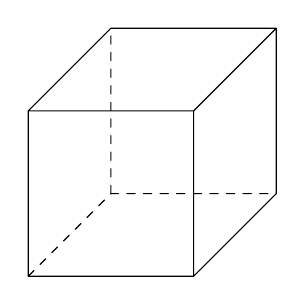
\begin{tikzpicture}[scale=0.7, font=\footnotesize, line join=round, line cap=round, >=stealth]
	\def\a{3} %chiều cao
	\path
	(0,0) coordinate (A) 
	(\a,0) coordinate (B) 
	(1.5,1.5) coordinate (D) 
	(D)+(\a,0) coordinate (C);
	\foreach \x in {A,B,C,D}
	\path (\x)+(0,\a) coordinate(\x1);	
	\draw[dashed] (A)--(D)--(C) (D)--(D1);
	\draw(A1)--(B1)--(C1)--(D1)--(A1)--(A)--(B)--(C)--(C1) (B)--(B1);
	\end{tikzpicture}}
	\loigiai{
	Gọi $x$ (dm, $x>0$) là độ dài cạnh của thùng hình lập phương cần làm.\\
	Ta có $x^{3}=216$, suy ra $x=\sqrt[3]{216}=6$ (dm).\\
	Vì thùng đựng không có nắp nên thùng gồm $4$ mặt bên và $1$ mặt đáy, mỗi mặt là một hình vuông cạnh $6$ dm. Do đó diện tích bìa cứng cần dùng là
	\begin{center}
	$S=5 \cdot 6^{2}=180.$ ({dm}$^{2}$)
	\end{center}
	}
\end{bt}